\documentclass[10pt,aspectratio=169]{beamer}

% --- Preamble ---
\usetheme{CambridgeUS}
\usecolortheme{beaver}
\usepackage[utf8]{inputenc}
\usepackage[english]{babel}
\usepackage{amsmath}
\usepackage{amsfonts}
\usepackage{amssymb}
\usepackage{graphicx}
\usepackage{booktabs}
\usepackage{xcolor}
\usepackage{pifont}
\usepackage{tikz}
\usetikzlibrary{positioning, shapes, arrows.meta, calc}
\graphicspath{{pics/}}
\usepackage{etoolbox}

% --- Make framesubtitle clearly distinct (dark gray, not red) ---
\setbeamercolor{framesubtitle}{fg=darkgray}
\setbeamerfont{framesubtitle}{size=\normalsize, series=\mdseries}

% --- Enhanced navigation bar ---
\setbeamerfont{section in head/foot}{series=\bfseries}
\setbeamertemplate{navigation symbols}{}  % Remove tiny nav icons

% --- Frame counter in footer ---
\setbeamertemplate{footline}{%
  \leavevmode%
  \hbox{%
    \begin{beamercolorbox}[wd=.333\paperwidth,ht=2.25ex,dp=1ex,center]{author in head/foot}%
      \usebeamerfont{author in head/foot}\insertshortauthor
    \end{beamercolorbox}%
    \begin{beamercolorbox}[wd=.333\paperwidth,ht=2.25ex,dp=1ex,center]{title in head/foot}%
      \usebeamerfont{title in head/foot}\insertshorttitle
    \end{beamercolorbox}%
    \begin{beamercolorbox}[wd=.333\paperwidth,ht=2.25ex,dp=1ex,right]{date in head/foot}%
      \usebeamerfont{date in head/foot}\insertshortdate{}\hspace*{2em}
      \insertframenumber{} / \inserttotalframenumber\hspace*{2ex}
    \end{beamercolorbox}%
  }%
  \vskip0pt%
}

% --- Logo (shown on every slide footer) ---
\logo{
\includegraphics[height=0.5cm]{usth.png}}

% --- Metadata ---
\title[ANSER]{ANSER}
\subtitle{\normalsize \textit{Automated Nimble Software Easing Relaxation}\\[0.4cm]
\large A Solution For Retail Management Stores}
\author[Group 13 -  Group Project]{Group 13 --- ICT 3.019 Group Project}
\institute[USTH]{University of Science and Technology of Hanoi}
\date{April 07, 2026}

\begin{document}

% ═══════════════════════════════════════════════════════════════
% SLIDE 1: Title Page
% ═══════════════════════════════════════════════════════════════
\begin{frame}
    \titlepage
\end{frame}

% ═══════════════════════════════════════════════════════════════
% SLIDE 2: Group Members
% ═══════════════════════════════════════════════════════════════
\begin{frame}{Group Members}
    \centering
    \vspace{0.3cm}
    \begin{tabular}{c l l}
        \textbf{\#} & \textbf{Student ID} & \textbf{Full Name} \\
        \hline
        \rule{0pt}{2.5ex}1 & 23BI14386 & Hà Thái Sơn \\
        2 & 23BI14279 & Phạm Thế Minh \\
        3 & 23BI14396 & Trần Quốc Thái \\
        4 & 23BI14444 & Phạm Ngọc Tùng \\
        5 & 23BI14342 & Nguyễn Duy Ngọc \\
        6 & 23BI14388 & Nghiêm Xuân Sơn \\
        7 & 23BI14303 & Trần Vũ Công Minh \\
    \end{tabular}
    \vspace{0.5cm}

    \textbf{Supervisor:} Mr.\ Dao Thuong Huong
\end{frame}

% ═══════════════════════════════════════════════════════════════
% SLIDE 3: Agenda
% ═══════════════════════════════════════════════════════════════
\begin{frame}{Agenda}
    \tableofcontents
\end{frame}

% ===========================================================
\section{1. Introduction}
% ===========================================================

% ═══════════════════════════════════════════════════════════════
% SLIDE 4: Problem & Motivation
% ═══════════════════════════════════════════════════════════════
\begin{frame}{1. Introduction}
    \framesubtitle{Problem \& Motivation}

    \begin{block}{The Challenge --- Vietnamese Retail SMEs}
        1.4M+ small retailers still rely on \textbf{paper invoices}, handwritten ledgers, and disconnected spreadsheets. Manual import cycles cause data drift, errors, and wasted labour.
    \end{block}
    \vspace{0.3cm}

    \textbf{Why existing platforms fall short:}
    \begin{itemize}
        \item \textbf{n8n / Make.com / Zapier} assume data is \emph{already digital}
        \item No native OCR --- cannot process a photograph of a paper invoice
        \item USD-denominated pricing is prohibitive for thin-margin Vietnamese shops
        \item Reliance on browser translation causes context loss and breaks financial data formatting
        \item Workflow construction requires technical expertise most operators lack
    \end{itemize}

    \vfill
    \begin{block}{Problem Statement}
        How can a \textbf{low-cost, self-hosted} platform automate the paper-invoice-to-inventory pipeline \emph{without} requiring technical expertise?
    \end{block}
\end{frame}

% ═══════════════════════════════════════════════════════════════
% SLIDE 5: ANSER Solution Overview
% ═══════════════════════════════════════════════════════════════
\begin{frame}{1. Introduction}
    \framesubtitle{ANSER --- RPAaaS for Vietnamese Retail}

    \textbf{Three Core Innovations:}
    \begin{enumerate}
        \item \textbf{Smart Import} --- Cascading OCR pipeline converts photographed paper invoices into structured JSON and updates inventory automatically.
        \item \textbf{Drag-and-Drop Workflow Engine} --- Visual DAG builder with Kahn's topological sort; 12 node types connecting Google Workspace, notifications, and DL services.
        \item \textbf{AI Agent} --- Translates natural language $\rightarrow$ executable workflow graphs, eliminating manual workflow construction.
    \end{enumerate}

    \vspace{0.3cm}
    \begin{table}
        \centering\footnotesize
        \begin{tabular}{lcccc}
            \toprule
            \textbf{Feature} & \textbf{n8n} & \textbf{Make.com} & \textbf{Zapier} & \textbf{ANSER} \\
            \midrule
            Self-hosted          & \checkmark & $\times$ & $\times$ & \checkmark \\
            Native OCR           & $\times$   & $\times$ & $\times$ & \checkmark \\
            Vietnamese support   & $\times$   & $\times$ & $\times$ & \checkmark \\
            AI workflow gen.     & $\times$   & Limited  & Limited  & \checkmark \\
            DAG execution        & \checkmark & \checkmark & $\times$ & \checkmark \\
            Free for SMEs        & \checkmark & $\times$ & $\times$ & \checkmark \\
            \bottomrule
        \end{tabular}
    \end{table}
\end{frame}

% ===========================================================
\section{2. System Architecture}
% ===========================================================

% ═══════════════════════════════════════════════════════════════
% SLIDE 6: System Architecture --- Three Microservices
% ═══════════════════════════════════════════════════════════════
\begin{frame}[fragile]{2. System Architecture}
    \framesubtitle{Three Independently Deployable Services}

    \begin{columns}
        \column{0.55\textwidth}
        \centering
        \scalebox{0.42}{%
        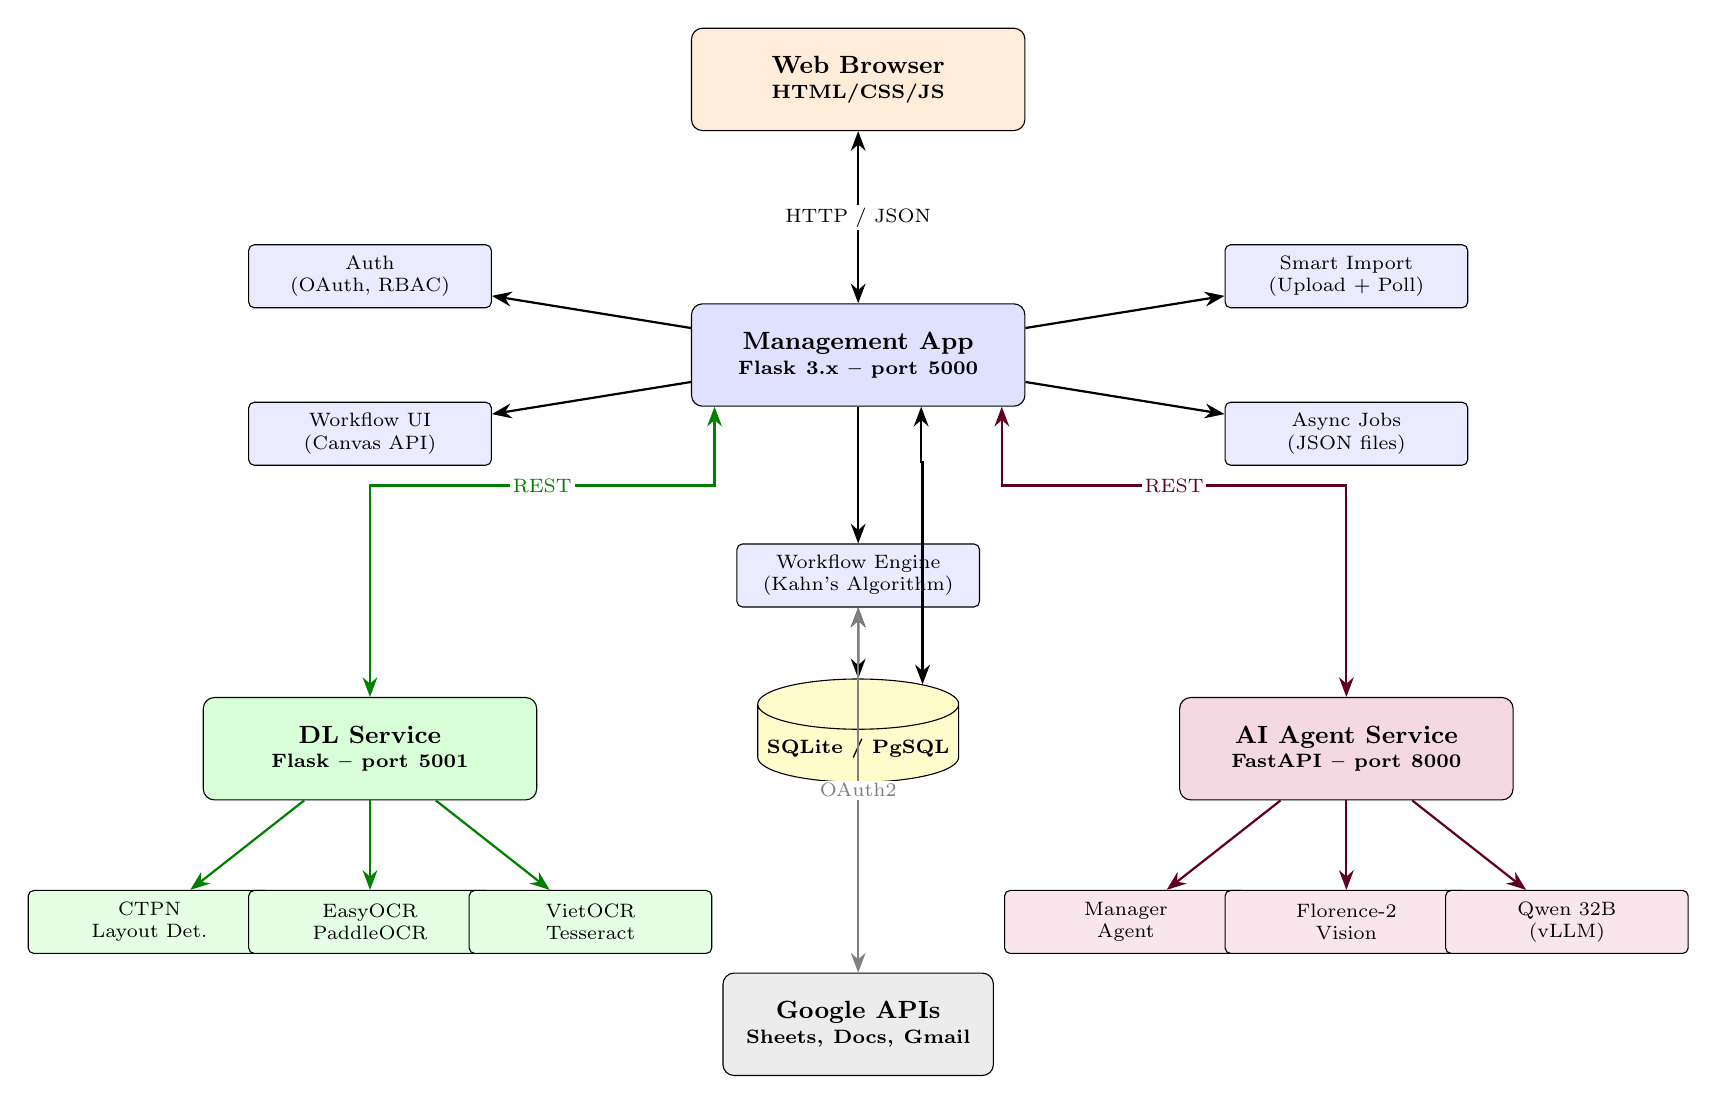
\begin{tikzpicture}[
          box/.style={draw, rounded corners=4pt, minimum height=1.3cm, text width=4cm, align=center, font=\small\bfseries, fill=#1},
          smallbox/.style={draw, rounded corners=2pt, minimum height=0.8cm, text width=2.8cm, align=center, font=\scriptsize, fill=#1, inner sep=4pt},
          dbcyl/.style={draw, cylinder, shape border rotate=90, minimum height=1.1cm, minimum width=1.8cm, aspect=0.25, font=\scriptsize\bfseries, fill=#1},
          arr/.style={-{Stealth[length=2.5mm]}, thick, #1},
          darr/.style={{Stealth[length=2.5mm]}-{Stealth[length=2.5mm]}, thick, #1},
          lbl/.style={font=\scriptsize, midway, fill=white, inner sep=1pt}
        ]
        \node[box=orange!15] (browser) at (0, 0.5) {Web Browser\\[-2pt]\scriptsize HTML/CSS/JS};
        \node[box=blue!12] (flask) at (0, -3) {Management App\\[-2pt]\scriptsize Flask 3.x -- port 5000};
        \node[smallbox=blue!8] (auth) at (-6.2, -2.0) {Auth\\(OAuth, RBAC)};
        \node[smallbox=blue!8] (wfui) at (-6.2, -4.0) {Workflow UI\\(Canvas API)};
        \node[smallbox=blue!8] (smart) at (6.2, -2.0) {Smart Import\\(Upload + Poll)};
        \node[smallbox=blue!8] (jobs) at (6.2, -4.0) {Async Jobs\\(JSON files)};
        \node[smallbox=blue!8] (wfeng) at (0, -5.8) {Workflow Engine\\(Kahn's Algorithm)};
        \node[dbcyl=yellow!20] (db) at (0, -8) {SQLite / PgSQL};
        \node[box=green!15] (dl) at (-6.2, -8) {DL Service\\[-2pt]\scriptsize Flask -- port 5001};
        \node[smallbox=green!10] (ctpn) at (-9, -10.2) {CTPN\\Layout Det.};
        \node[smallbox=green!10] (ocr) at (-6.2, -10.2) {EasyOCR\\PaddleOCR};
        \node[smallbox=green!10] (easy) at (-3.4, -10.2) {VietOCR\\Tesseract};
        \node[box=purple!15] (ai) at (6.2, -8) {AI Agent Service\\[-2pt]\scriptsize FastAPI -- port 8000};
        \node[smallbox=purple!10] (mgr) at (3.4, -10.2) {Manager\\Agent};
        \node[smallbox=purple!10] (flor) at (6.2, -10.2) {Florence-2\\Vision};
        \node[smallbox=purple!10] (qwen) at (9, -10.2) {Qwen 32B\\(vLLM)};
        \node[box=gray!15, text width=3.2cm] (gapi) at (0, -11.5) {Google APIs\\[-2pt]\scriptsize Sheets, Docs, Gmail};
        \draw[darr=black] (browser) -- node[lbl] {HTTP / JSON} (flask);
        \draw[arr=black] (flask) -- (auth);
        \draw[arr=black] (flask) -- (wfui);
        \draw[arr=black] (flask) -- (smart);
        \draw[arr=black] (flask) -- (jobs);
        \draw[arr=black] (flask) -- (wfeng);
        \draw[darr=black] (wfeng) -- (db);
        \draw[darr=green!50!black] (flask.south west) ++(0.3,0) -- ++(0,-1) -| node[lbl, pos=0.25] {REST} (dl.north);
        \draw[darr=purple!50!black] (flask.south east) ++(-0.3,0) -- ++(0,-1) -| node[lbl, pos=0.25] {REST} (ai.north);
        \draw[arr=green!50!black] (dl) -- (ctpn);
        \draw[arr=green!50!black] (dl) -- (ocr);
        \draw[arr=green!50!black] (dl) -- (easy);
        \draw[arr=purple!50!black] (ai) -- (mgr);
        \draw[arr=purple!50!black] (ai) -- (flor);
        \draw[arr=purple!50!black] (ai) -- (qwen);
        \draw[darr=gray] (wfeng) -- node[lbl] {OAuth2} (gapi);
        \draw[darr=black] (flask.south) ++(0.8,0) -- ++(0,-0.7) -| (db.north east);
        \end{tikzpicture}}

        \column{0.45\textwidth}
        \small
        \textbf{1.\ Management App} (Flask, port 5000):
        \begin{itemize}\small
            \item Auth, CRUD, Workflow UI, Smart Import
            \item Orchestrates all downstream calls
        \end{itemize}
        \vspace{0.2cm}
        \textbf{2.\ DL Service} (Flask, port 5001):
        \begin{itemize}\small
            \item CTPN layout detection (VGG-16)
            \item Cascading OCR: EasyOCR $\rightarrow$ PaddleOCR $\rightarrow$ VietOCR $\rightarrow$ Tesseract
        \end{itemize}
        \vspace{0.2cm}
        \textbf{3.\ AI Agent Service} (FastAPI, port 8000):
        \begin{itemize}\small
            \item Multi-agent: Manager, Coder, Vision, Researcher
            \item Qwen2.5-Coder-32B-AWQ (vLLM) + Florence-2
        \end{itemize}
        \vspace{0.2cm}
        \textbf{Database:} PostgreSQL(NeonDB)\\
        \texttt{PGShimCursor} --- zero app-code changes
    \end{columns}
\end{frame}

% ===========================================================
\section{3. Methodology}
% ===========================================================

% ═══════════════════════════════════════════════════════════════
% SLIDE 7: Smart Import Pipeline
% ═══════════════════════════════════════════════════════════════
\begin{frame}{3. Methodology}
    \framesubtitle{Smart Import --- Paper Invoice to Structured Data}

    \begin{columns}
        \column{0.5\textwidth}
        \begin{figure}
            \centering
            \includegraphics[width=\textwidth,height=0.55\textheight,keepaspectratio]{pics/importocr.jpg}
            \caption{Smart Import OCR: invoice uploaded, OCR extraction results displayed for human verification.}
        \end{figure}

        \column{0.5\textwidth}
        \small
        \textbf{Five-Stage Pipeline:}
        \begin{enumerate}
            \item \textbf{Upload} image (JPEG/PNG, $\leq$16\,MB)
            \item \textbf{CTPN} layout detection (VGG-16 backbone) isolates product table
            \item \textbf{Cascading OCR:}\\
                  EasyOCR $\rightarrow$ PaddleOCR $\rightarrow$ VietOCR $\rightarrow$ Brain VLM $\rightarrow$ Tesseract
            \item \textbf{Product Extraction:} regex parser for Vietnamese number formatting
            \item \textbf{Database Update:} inventory auto-incremented
        \end{enumerate}
        \vspace{0.2cm}
        \textbf{Human-in-the-loop:} user reviews pre-filled form before committing.
    \end{columns}
\end{frame}

% ═══════════════════════════════════════════════════════════════
% SLIDE 8: Workflow Engine --- Kahn's Algorithm
% ═══════════════════════════════════════════════════════════════
\begin{frame}[fragile]{3. Methodology}
    \framesubtitle{Drag-and-Drop Workflow Engine --- Kahn's Algorithm}

    \begin{columns}
        \column{0.5\textwidth}
        \centering
        % Kahn's Algorithm DAG trace (from report Fig 4.4)
        \scalebox{0.55}{%
        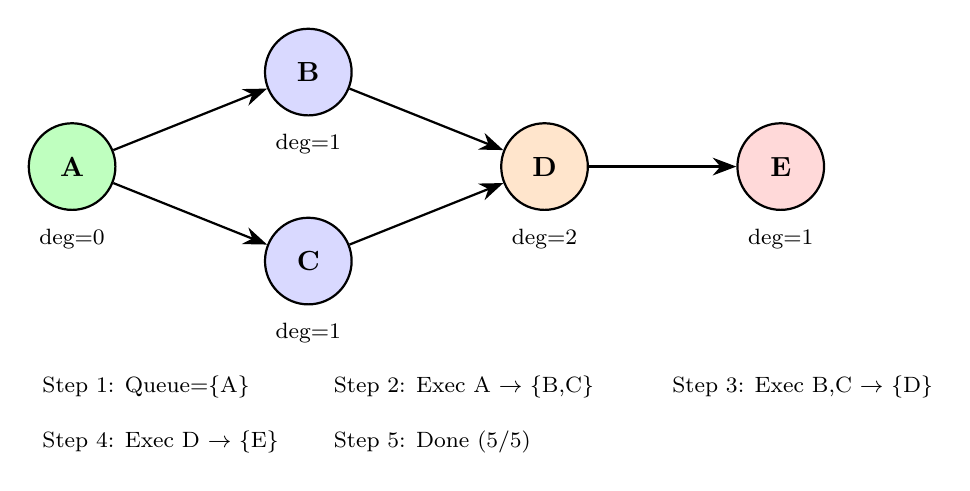
\begin{tikzpicture}[
          nd/.style={draw, circle, minimum size=1.1cm, font=\normalsize\bfseries, fill=#1, line width=0.8pt},
          edg/.style={-{Stealth[length=3mm]}, thick},
        ]
        \node[nd=green!25] (A) at (0,0) {A};
        \node[nd=blue!15]  (B) at (3,1.2) {B};
        \node[nd=blue!15]  (C) at (3,-1.2) {C};
        \node[nd=orange!20](D) at (6,0) {D};
        \node[nd=red!15]   (E) at (9,0) {E};
        \draw[edg] (A) -- (B);
        \draw[edg] (A) -- (C);
        \draw[edg] (B) -- (D);
        \draw[edg] (C) -- (D);
        \draw[edg] (D) -- (E);
        \node[font=\footnotesize, below=3pt] at (A.south) {deg=0};
        \node[font=\footnotesize, below=3pt] at (B.south) {deg=1};
        \node[font=\footnotesize, below=3pt] at (C.south) {deg=1};
        \node[font=\footnotesize, below=3pt] at (D.south) {deg=2};
        \node[font=\footnotesize, below=3pt] at (E.south) {deg=1};
        % Execution trace — placed BELOW graph to avoid right-column overlap
        \node[font=\footnotesize, anchor=west] at (-0.5,-2.8) {Step 1: Queue=$\lbrace$A$\rbrace$};
        \node[font=\footnotesize, anchor=west] at (3.2,-2.8) {Step 2: Exec A $\to$ $\lbrace$B,C$\rbrace$};
        \node[font=\footnotesize, anchor=west] at (7.5,-2.8) {Step 3: Exec B,C $\to$ $\lbrace$D$\rbrace$};
        \node[font=\footnotesize, anchor=west] at (-0.5,-3.5) {Step 4: Exec D $\to$ $\lbrace$E$\rbrace$};
        \node[font=\footnotesize, anchor=west] at (3.2,-3.5) {Step 5: Done (5/5)};
        \end{tikzpicture}}
        \vspace{0.15cm}
        \includegraphics[width=0.95\textwidth,height=0.25\textheight,keepaspectratio]{node.png}

        \column{0.5\textwidth}
        \small
        \textbf{Workflow = DAG} (Directed Acyclic Graph):
        \begin{itemize}
            \item \textbf{Nodes} = actions (read sheet, send email, run OCR\ldots)
            \item \textbf{Edges} = data-flow dependencies
        \end{itemize}
        \vspace{0.2cm}
        \textbf{Kahn's Algorithm} (Topological sort):
        \begin{itemize}
            \item Time Complexity: $O(V+E)$
            \item Detects cycles before execution
            \item Context propagation via \texttt{\{\{node\_id.field\}\}} templates
        \end{itemize}
    \end{columns}
\end{frame}

% ═══════════════════════════════════════════════════════════════
% SLIDE 8b: Workflow Engine --- 12 Node Types
% ══════════════════════════════════════════════════════════

% ═══════════════════════════════════════════════════════════════
% SLIDE 9: AI Agent --- Multi-Agent + NL to Workflow
% ═══════════════════════════════════════════════════════════════
\begin{frame}{3. Methodology}
    \framesubtitle{AI Agent --- Natural Language to Executable Workflows}

    \begin{columns}
        \column{0.5\textwidth}
        \textbf{Multi-Agent Architecture:}
        \begin{itemize}
            \item \textbf{ManagerAgent}: Hybrid router (RegEx fast-path + LLM classification). Delegates to specialists.
            \item \textbf{CoderAgent}: Generates executable JSON DAGs from natural language.
            \item \textbf{VisionAgent}: Florence-2-large for image understanding (scene description, OCR).
            \item \textbf{ResearcherAgent}: RAG (ChromaDB) + web search for factual queries.
        \end{itemize}

        \column{0.5\textwidth}
        \textbf{Natural Language $\rightarrow$ Workflow Translation:}\\[0.2cm]
        User says: \textit{``Read the sales sheet and email summary to management.''}\\
        {\scriptsize(Vietnamese demo prompt: Appendix~A)}

        \vspace{0.2cm}
        $\downarrow$ ManagerAgent classifies as \texttt{TECHNICAL}

        $\downarrow$ CoderAgent generates JSON DAG
        
        \vspace{0.2cm}
        \normalsize
        $\downarrow$ Workflow Engine executes via Kahn's.

       
    \end{columns}
\end{frame}

% ===========================================================
\section{4. Implementation \& User Interface}
% ===========================================================

% ═══════════════════════════════════════════════════════════════
% ═══════════════════════════════════════════════════════════════
% SLIDE 10: Admin Dashboard + Smart Import
% ═══════════════════════════════════════════════════════════════
\begin{frame}{4. Implementation \& User Interface}
    \framesubtitle{Administrator Dashboard}

    \begin{columns}
        \column{0.5\textwidth}
        \begin{figure}
            \centering
            \includegraphics[width=\textwidth,height=0.6\textheight,keepaspectratio]{admin_dashboard.jpg}
            \caption{Admin Analytics Dashboard.}
        \end{figure}

        \column{0.5\textwidth}
        \textbf{Platform Security \& Control:}
        \begin{itemize}
            \item \textbf{Access Control (RBAC):}\\ Strict view separation (Admin vs.\ Employee) via Jinja2 SSR.
            \item \textbf{System Telemetry:}\\ Real-time monitoring of active user sessions.
            \item \textbf{Secure CRUD:}\\ All database operations parameterized via \texttt{PGShimCursor} to prevent SQL injection.
        \end{itemize}
    \end{columns}
\end{frame}

% ═══════════════════════════════════════════════════════════════
% SLIDE 10b: Smart Import UI
% ═══════════════════════════════════════════════════════════════
\begin{frame}{4. Implementation \& User Interface}
    \framesubtitle{Smart Import --- Upload to Inventory}

    \begin{columns}
        \column{0.5\textwidth}
        \begin{figure}
            \centering
            \includegraphics[width=\textwidth,height=0.6\textheight,keepaspectratio]{pics/Import.jpg}
            \caption{Smart Import verification interface.}
        \end{figure}

        \column{0.5\textwidth}
        \textbf{Pipeline Integration:}
        \begin{itemize}
            \item \textbf{Microservice Proxy:}\\ Main app validates and forwards uploads to the isolated DL Service.
            \item \textbf{Human-in-the-Loop:}\\ OCR JSON pre-fills editable forms for operator review before atomic DB commits.
            
        \end{itemize}
    \end{columns}
\end{frame}

% ═══════════════════════════════════════════════════════════════
% SLIDE 11: AI Agent Chat + Workflow Builder
% ═══════════════════════════════════════════════════════════════
\begin{frame}{4. Implementation \& User Interface}
    \framesubtitle{AI Agent --- Natural Language to Workflow}

    \begin{columns}
        \column{0.5\textwidth}
        \begin{figure}
            \centering
            \includegraphics[width=\textwidth,height=0.55\textheight,keepaspectratio]{ai_workflow_succeed.jpg}
            \caption{AI Agent generating workflow nodes to workspace.}
        \end{figure}

        \column{0.5\textwidth}
        \textbf{UI \& Agent Integration:}
        \begin{itemize}
            \item \textbf{Non-Blocking UX:}\\ Asynchronous background processing keeps the browser highly responsive and prevents freezing during LLM inference (5--30\,s).
            \item \textbf{Dynamic Canvas Rendering:}\\ The AI's output is instantly visualized on the HTML5 Canvas, allowing intuitive, human-in-the-loop editing before execution.
        \end{itemize}
    \end{columns}
\end{frame}

% ═══════════════════════════════════════════════════════════════
% SLIDE 11b: End-to-End Workflow Execution
% ═══════════════════════════════════════════════════════════════
\begin{frame}{4. Implementation \& User Interface}
    \framesubtitle{End-to-End Execution --- Workflow Automation}

    \begin{columns}
        \column{0.33\textwidth}
        \begin{figure}
            \centering
            \includegraphics[width=\textwidth,height=0.55\textheight,keepaspectratio]{source_docs.jpg}
            \caption{Input: Google Docs.}
        \end{figure}

        \column{0.33\textwidth}
        \begin{figure}
            \centering
            \includegraphics[width=\textwidth,height=0.55\textheight,keepaspectratio]{workflow_succeed_manual.jpg}
            \caption{Workflow execution.}
        \end{figure}

        \column{0.33\textwidth}
        \begin{figure}
            \centering
            \includegraphics[width=\textwidth,height=0.55\textheight,keepaspectratio]{result_gmail.png}
            \caption{Output: automated Gmail.}
        \end{figure}
    \end{columns}

    \vspace{0.2cm}
    \centering\small
    The workflow automation executed successfully: Kahn's topological sort $\to$ resolve templates $\to$ dispatch Google API calls $\to$ propagate context.
\end{frame}

% ===========================================================
\section{5. Evaluation}
% ===========================================================

% ═══════════════════════════════════════════════════════════════
% SLIDE 12: Pillar 1 --- Data Mapping Accuracy
% ═══════════════════════════════════════════════════════════════
% ═══════════════════════════════════════════════════════════════
% SLIDE 12: Pillar 1 --- Data Mapping Accuracy
% ═══════════════════════════════════════════════════════════════
% ═══════════════════════════════════════════════════════════════
% SLIDE 12: Pillar 1 --- Data Mapping Accuracy
% ═══════════════════════════════════════════════════════════════
\begin{frame}{5. Evaluation}
  \framesubtitle{Pillar 1 --- Data Mapping Accuracy (30 synthetic test images)}

  \begin{columns}[t]
    \column{0.48\textwidth}
    \begin{table}
      \centering\scriptsize
      \begin{tabular}{lc}
        \toprule
        \textbf{Metric} & \textbf{Value} \\
        \midrule
        \multicolumn{2}{l}{\emph{Pipeline infrastructure}} \\
        Layout Detection (CTPN)  & \textbf{100.0\%} \\
        OCR Text Extraction      & \textbf{100.0\%} \\
        Avg Detection Confidence & 95.8\% \\
        Avg OCR Confidence       & 89.5\% \\
        \midrule
        \multicolumn{2}{l}{\emph{Field-level (synthetic gap)}} \\
        Quantity Accuracy         & 50.0\% \\
        Price Accuracy            & 6.4\% \\
        Product Name Match        & 2.8\% \\
        Pipeline Completion       & 86.7\% \\
        \bottomrule
      \end{tabular}
      \caption{Smart Import results. \newline
      Dataset: 1,200 synthetic images, 15,420 SKUs.}
    \end{table}

    \column{0.48\textwidth}
    \textbf{Key Findings:}
    \begin{itemize}
      \item \textbf{Architecture Validated:}\\ CTPN + Cascading OCR achieved \textbf{100\%} region detection and text extraction.
      \vspace{0.2cm}
      \item \textbf{Synthetic Domain Gap:}\\ Real-world-trained models struggled on synthetic PIL-rendered fonts; digits extracted at $18\times$ the rate of Vietnamese text (50\% vs.\ 2.8\%).
      \vspace{0.2cm}
      \item \textbf{Production Viability:}\\ 86.7\% usable field yield confirms Human-in-the-Loop pre-fill is effective for assisted data entry.
    \end{itemize}
  \end{columns}
\end{frame}


% ═══════════════════════════════════════════════════════════════
% SLIDE 13: Pillar 2 + 3 --- Latency + Routing
% ═══════════════════════════════════════════════════════════════
\begin{frame}{5. Evaluation}
    \framesubtitle{Pillar 2 --- Execution Latency \& Pillar 3 --- Workflow Routing Accuracy}

    \begin{columns}
        \column{0.5\textwidth}
        \textbf{Pillar 2: Execution Latency}
        \begin{table}
            \centering\footnotesize
            \begin{tabular}{lc}
                \toprule
                \textbf{Operation} & \textbf{Mean} \\
                \midrule
                Smart Import (CPU) & 2,480\,ms \\
                Kahn's (5 nodes)   & 2.0\,$\mu$s \\
                Kahn's (10 nodes)  & 4.9\,$\mu$s \\
                Kahn's (50 nodes)  & 19.3\,$\mu$s \\
                Kahn's (100 nodes) & 38.5\,$\mu$s \\
                \bottomrule
            \end{tabular}
        \end{table}
        \small
        Scheduling overhead is \textbf{negligible}. Bottleneck is I/O-bound node execution (API calls), not the algorithm.\\
        GPU deployment reduces OCR to $<$1\,s.

        \column{0.5\textwidth}
        \textbf{Pillar 3: Workflow Routing (16 Vietnamese prompts)}
        \begin{table}
            \centering\footnotesize
            \begin{tabular}{lcc}
                \toprule
                \textbf{Category} & \textbf{F1} & \textbf{n} \\
                \midrule
                Technical    & 1.00 & 4 \\
                Data Internal & 0.89 & 4 \\
                Marketing    & 1.00 & 4 \\
                General      & 0.86 & 4 \\
                \midrule
                \textbf{Weighted Avg} & \textbf{0.94} & \textbf{16} \\
                \bottomrule
            \end{tabular}
        \end{table}
        \small
        Workflow engine: \textbf{100\%} valid JSON parse, \textbf{100\%} cycle detection. 40\% full execution rate.
    \end{columns}
\end{frame}

% ===========================================================
\section{6. Security}
% ===========================================================

% ═══════════════════════════════════════════════════════════════
% SLIDE 14: Pentest Results
% ═══════════════════════════════════════════════════════════════
\begin{frame}{6. Security}
    \framesubtitle{Application Security Stack}

    \begin{columns}
        \column{0.5\textwidth}
        \textbf{Authentication \& Authorization:}
        \begin{itemize}
            \item Google OAuth 2.0 + OIDC (Authlib)
            \item Offline refresh tokens for API access
            \item RBAC: Admin $\to$ Manager $\to$ Employee
            \item Werkzeug password hashing (bcrypt)
        \end{itemize}

        \vspace{0.3cm}
        \textbf{Input Validation:}
        \begin{itemize}
            \item \texttt{PGShimCursor}: parameterized queries (prevents SQLi)
            \item Flask-WTF CSRF tokens on all state-changing requests
            \item File type \& size validation ($\leq$16\,MB)
        \end{itemize}

        \column{0.5\textwidth}
        \textbf{HTTP Security (Flask-Talisman):}
        \begin{itemize}
            \item Strict-Transport-Security (HSTS)
            \item X-Frame-Options: \texttt{DENY}
            \item X-Content-Type-Options: \texttt{nosniff}
            \item Content-Security-Policy (per-directive)
            \item Secure session cookies
        \end{itemize}

        \vspace{0.3cm}
        \textbf{Rate Limiting (Flask-Limiter):}
        \begin{itemize}
            \item Default: 20,000/day, 5,000/hour
            \item Per-endpoint customization
            \item Brute-force protection
        \end{itemize}
    \end{columns}

    \vspace{0.3cm}
    \centering\small
    \textit{Penetration test results: Appendix~B. Zero application-layer vulnerabilities found.}
\end{frame}

% ===========================================================
\section{7. Conclusion}
% ===========================================================

% ═══════════════════════════════════════════════════════════════
% SLIDE 15: Conclusion
% ═══════════════════════════════════════════════════════════════
\begin{frame}{7. Conclusion \& Future Work}

    \begin{block}{Contributions}
        \begin{enumerate}
            \item \textbf{Smart Import Pipeline}: Cascading OCR (CTPN + EasyOCR/PaddleOCR/VietOCR/Tesseract) and human-in-the-loop verification.
            \item \textbf{Drag-and-Drop Workflow Engine}: 12 node types, Kahn's algorithm, context propagation via template variables.
            \item \textbf{AI Agent}: Natural Language $\rightarrow$ executable JSON DAGs via Qwen2.5-Coder-32B-AWQ. 
            \item \textbf{Three-Pillar Evaluation}: Data Mapping Accuracy, Execution Latency, Workflow Routing Accuracy.
        \end{enumerate}
    \end{block}

    \vspace{0.2cm}
    \begin{block}{Future Work}
        \begin{itemize}
            \item Fine-tuned OCR on real Vietnamese invoices (close the synthetic domain gap)
            \item Mobile app for invoice capture and workflow monitoring
        \end{itemize}
    \end{block}
\end{frame}

% ═══════════════════════════════════════════════════════════════
% SLIDE 16: Live Demo Transition
% ═══════════════════════════════════════════════════════════════
\begin{frame}{}
    \centering
    \vspace{1.5cm}
    {\Huge\bfseries Live Demo}\\[0.5cm]
    {\large Smart Import - Workflow Builder - AI Agent Chat}\\[1cm]
\end{frame}

% ═══════════════════════════════════════════════════════════════
% SLIDE 17: References
% ═══════════════════════════════════════════════════════════════
\begin{frame}{References}
    \tiny
    \begin{columns}[T]
        \column{0.5\textwidth}
        \textbf{OCR \& Vision}
        \begin{enumerate}
            \item[{[1]}] Smith, R. (2007). \textit{An overview of the Tesseract OCR engine.} ICDAR.
            \item[{[2]}] Du, Y. et al. (2020). \textit{PP-OCR: A practical ultra lightweight OCR system.} arXiv:2009.09941.
            \item[{[3]}] Tian, Z. et al. (2016). \textit{Detecting text in natural image with CTPN.} ECCV.
            \item[{[4]}] pbcquoc (2021). \textit{VietOCR: Transformer-based Vietnamese OCR.} github.com/pbcquoc/vietocr.
            \item[{[5]}] JaidedAI (2020). \textit{EasyOCR: Ready-to-use OCR with 80+ languages.} github.com/JaidedAI/EasyOCR.
            \item[{[6]}] PaddlePaddle (2023). \textit{PaddleOCR: Multilingual OCR toolkits.} github.com/PaddlePaddle/PaddleOCR.
            \item[{[7]}] Simonyan, K. \& Zisserman, A. (2015). \textit{Very deep convolutional networks (VGGNet).} ICLR.
            \item[{[8]}] Baviskar, D. et al. (2021). \textit{End-to-end methods for document invoice processing.} IEEE Access.
        \end{enumerate}
        \vspace{0.05cm}
        \textbf{LLMs \& Agents}
        \begin{enumerate}
            \item[{[9]}] Xiao, B. et al. (2023). \textit{Florence-2: Advancing a unified representation.} arXiv:2311.06242.
            \item[{[10]}] Hui, B. et al. (2024). \textit{Qwen2.5-Coder technical report.} arXiv:2409.12186.
            \item[{[11]}] Kwon, W. et al. (2023). \textit{vLLM: Easy, fast, cheap LLM serving with PagedAttention.} SOSP.
            \item[{[12]}] Yao, S. et al. (2023). \textit{ReAct: Synergizing reasoning and acting in LMs.} ICLR.
            \item[{[13]}] ChromaDB (2024). \textit{Open-source embedding database.} trychroma.com.
        \end{enumerate}

        \column{0.5\textwidth}
        \textbf{Retail \& Automation}
        \begin{enumerate}
            \item[{[14]}] van der Aalst, W. et al. (2018). \textit{Robotic process automation.} Bus. \& IS Eng.
            \item[{[15]}] Munoz Macas, C.V. et al. (2021). \textit{Inventory management for retail: a lit. review.}
        \end{enumerate}
        \vspace{0.05cm}
        \textbf{Workflow \& Architecture}
        \begin{enumerate}
            \item[{[16]}] Kahn, A.B. (1962). \textit{Topological sorting of large networks.} CACM, 5(11).
            \item[{[17]}] Georgakopoulos, D. et al. (1995). \textit{An overview of workflow management.}
            \item[{[18]}] Newman, S. (2015). \textit{Building Microservices.} O'Reilly.
            \item[{[19]}] n8n.io (2024). Self-hosted workflow automation.
            \item[{[20]}] Make.com (2024). Visual automation platform.
            \item[{[21]}] Zapier (2024). Workflow automation for everyone.
        \end{enumerate}
        \vspace{0.05cm}
        \textbf{Web Frameworks \& Security}
        \begin{enumerate}
            \item[{[22]}] Pallets Projects (2024). \textit{Flask: web development, one drop at a time.}
            \item[{[23]}] Google (2024). \textit{Google API Python Client.} github.com/googleapis.
            \item[{[24]}] OWASP (2021). \textit{OWASP Top 10 --- 2021.}
            \item[{[25]}] GSO Vietnam (2023). \textit{Statistical yearbook of Vietnam.}
        \end{enumerate}
        \vspace{0.05cm}
    \end{columns}
\end{frame}

% ═══════════════════════════════════════════════════════════════
% SLIDE 18: Q&A
% ═══════════════════════════════════════════════════════════════
\begin{frame}{Q\&A}
    \centering
    \vspace{1cm}
    \Large \textbf{Thank You --- Questions?}
    \vspace{0.5cm}

    \normalsize
    \textbf{ANSER}: Robotic Process Automation as a Service\\
    for Vietnamese Retail SMEs\\[0.5cm]
    \small
    Smart Import $\cdot$ Workflow Engine $\cdot$ AI Agent
\end{frame}

% ===========================================================
% APPENDIX (supplementary slides — not counted in main presentation)
% ===========================================================
\appendix

% ═══════════════════════════════════════════════════════════════
% APPENDIX A: Vietnamese Prompt Example
% ═══════════════════════════════════════════════════════════════
\begin{frame}{Appendix A: Vietnamese Prompt Example}
    \small
    \textbf{Real user prompt (Vietnamese):}
    \vspace{0.3cm}

    \begin{exampleblock}{Input}
        \textit{``Tôi muốn làm 1 quy trình tự động hóa mà nó sẽ tự đọc file Google Sheet `Kịch bản' và gửi email về kịch bản đó cho email: sonkhagioi@gmail.com.''}
    \end{exampleblock}

    \vspace{0.3cm}
    \textbf{AI Agent Pipeline:}
    \begin{enumerate}
        \item ManagerAgent classifies $\to$ \texttt{TECHNICAL}
        \item CoderAgent generates JSON DAG:
            \begin{itemize}
                \item \texttt{node\_1: google\_sheet\_read} (source: ``Kịch bản'')
                \item \texttt{node\_2: gmail\_send} (to: sonkhagioi@gmail.com)
                \item \texttt{edge: node\_1 $\to$ node\_2}, body: \texttt{\{\{node\_1.data\}\}}
            \end{itemize}
        \item Workflow Engine executes via Kahn's algorithm
    \end{enumerate}

    \vspace{0.2cm}
    \textit{English: ``I want an automation that reads Google Sheet `Kịch bản' and emails its content to sonkhagioi@gmail.com.''}
\end{frame}

% ═══════════════════════════════════════════════════════════════
% APPENDIX B: Penetration Test Results
% ═══════════════════════════════════════════════════════════════
\begin{frame}{Appendix B: Penetration Test Summary}

    \small
    \begin{table}
        \centering
        \begin{tabular}{lcp{7.5cm}}
            \toprule
            \textbf{Severity} & \textbf{Count} & \textbf{Status} \\
            \midrule
            High   & 1 & Nginx 1.18.0 version CVE --- upgraded to $\geq$1.25.x \\
            Medium & 2 & Session cookie flags + CSP tightened \\
            Low    & 3 & HSTS preload, fingerprinting --- patched \\
            Info   & 3 & Informational findings --- resolved \\
            \midrule
            \multicolumn{3}{l}{\textbf{Application-layer result: 0 vulnerabilities}} \\
            \multicolumn{3}{l}{SQL injection, XSS, command injection: all clean.} \\
            \bottomrule
        \end{tabular}
    \end{table}

    \vspace{0.3cm}
    \centering
    All findings were \textbf{infrastructure-level} (Nginx web server).\\
    Application code passed penetration testing with \textbf{zero vulnerabilities}.
\end{frame}

\end{document}